\usepgflibrary{shapes.misc}
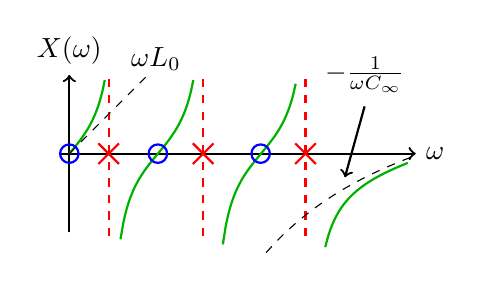
\begin{tikzpicture}[smooth, xscale=0.5, yscale=0.5]
% Achsen
\draw[->, thick] (-0.2,0) -- +(9,0) node[right] {$\omega$}; % Horizontal
\draw[->, thick] (0,-2) -- +(0,4) node[above] {$X(\omega)$}; % Vertikal

% Plots
\draw[color=green!70!black, thick] plot[domain=0.01:0.9] (\x, {tan( (\x *1.2) r )        }); % Erster Tan
\draw[color=green!70!black, thick] plot[domain=1.3:3.15] (\x,    {tan( (\x*1.2 -2.7) r)    }); % Erster Tan
\draw[color=green!70!black, thick] plot[domain=3.9:5.75] (\x,  {tan( (\x*1.2 -2.7) r)  }); % zweiter Tan
\draw[color=green!70!black, thick] plot[domain=6.5:8.6] (\x,  { ((0.25 * \x) -1/(\x -6)) -2 }); % letzte kurve

% Poolstellen
\draw[dashed, thick, draw=red] (1,-2.1) -- +(0,4.2); % Poolstelle 1
\node[cross out, draw=red, thick] at (1,0) {};

\draw[dashed, thick, draw=red] (3.4,-2.1) -- +(0,4.2); % Poolstelle 2
\node[cross out, draw=red, thick] at (3.4,0) {};

\draw[dashed, thick, draw=red] (6,-2.1) -- +(0,4.2); % Poolstelle 3
\node[cross out, draw=red, thick] at (6,0) {};

%\node[cross out, draw=red, thick] at (0,0) {};


\draw[dashed] plot[domain=5:8.7] (\x, { (-1 /(0.035 * \x)) + 3.2 });
\node (wC) at (7.5,2) {$- \frac{1}{\omega C_\infty}$};
\draw[->, thick] (7.5,1.2) -- +(-0.5,-1.8);

\draw[dashed] plot[domain=0:2] (\x,{\x});
\node at (2.2,2.4) {$\omega L_0$};


% Nullstellen
\node[rounded rectangle, draw=blue, thick] at(0,0) {};
\node[rounded rectangle, draw=blue, thick] at(2.25,0) {};
\node[rounded rectangle, draw=blue, thick] at(4.86,0) {};
\end{tikzpicture}